
%%%%%%%%%%%%%%%%%%%%%%% file typeinst.tex %%%%%%%%%%%%%%%%%%%%%%%%%
%
% This is the LaTeX source for the instructions to authors using
% the LaTeX document class 'llncs.cls' for contributions to
% the Lecture Notes in Computer Sciences series.
% http://www.springer.com/lncs       Springer Heidelberg 2006/05/04
%
% It may be used as a template for your own input - copy it
% to a new file with a new name and use it as the basis
% for your article.
%
% NB: the document class 'llncs' has its own and detailed documentation, see
% ftp://ftp.springer.de/data/pubftp/pub/tex/latex/llncs/latex2e/llncsdoc.pdf
%
%%%%%%%%%%%%%%%%%%%%%%%%%%%%%%%%%%%%%%%%%%%%%%%%%%%%%%%%%%%%%%%%%%%


\documentclass[runningheads,a4paper]{llncs}

\usepackage{amssymb}
\setcounter{tocdepth}{3}
\usepackage{graphicx}


\usepackage{listings}
\usepackage{upquote}
\usepackage{paralist}
\usepackage{commath}
\usepackage{enumerate}
%\usepackage[cmex10]{amsmath}
%\usepackage[pdftex]{graphicx}
\usepackage{amssymb}
\usepackage[caption=false,font=footnotesize]{subfig}

\usepackage{url}
\urldef{\mailsa}\path|{mohamed.abbadi, francesco.digiacomo, cortesi}@unive.it|
\urldef{\mailsb}\path|p.spronck@uvt.nl|
\urldef{\mailsc}\path|{costg,maggg}@hr.nl|
\newcommand{\keywords}[1]{\par\addvspace\baselineskip
\noindent\keywordname\enspace\ignorespaces#1}

\begin{document}

\mainmatter  % start of an individual contribution

% first the title is needed
\title{Casanova: A simple, high-performance language for game development}

% a short form should be given in case it is too long for the running head
\titlerunning{Casanova: A simple, high-performance language for game development}

% the name(s) of the author(s) follow(s) next
%
% NB: Chinese authors should write their first names(s) in front of
% their surnames. This ensures that the names appear correctly in
% the running heads and the author index.
%
\author{Mohamed Abbadi, Francesco Di Giacomo, Agostino Cortesi\\Pieter Spronck, Giulia Costantini, Giuseppe Maggiore}
%
\authorrunning{Mohamed Abbadi, Francesco Di Giacomo, Agostino Cortesi\\Pieter Spronck, Giulia Costantini, Giuseppe Maggiore}
% (feature abused for this document to repeat the title also on left hand pages)

% the affiliations are given next; don't give your e-mail address
% unless you accept that it will be published
\institute{Universit\`a Ca' Foscari DAIS, Venice, Italy\\
Tilburg University, Tilburg, Netherlands\\
Hogeschool Rotterdam, Rotterdam, Netherlands\\
\mailsa\\
\mailsb\\
\mailsc\\
\url{http://casanova.codeplex.com/}}

%
% NB: a more complex sample for affiliations and the mapping to the
% corresponding authors can be found in the file "llncs.dem"
% (search for the string "\mainmatter" where a contribution starts).
% "llncs.dem" accompanies the document class "llncs.cls".
%

\maketitle



\begin{abstract}
Managing the flow of time and the coordination of multiple components in games (and other highly interactive applications) is a challenging task. Therefore game development requires a lot of effort, even for (apparently) simple scenarios. To reduce the cost and effort of game development, we designed a new computer language called ``Casanova 2''. Using a case study, we demonstrate that Casanova 2 can be used to implement typical game scenario's using functional programming constructs. Our evaluation shows that it has both a high performance and a high usability.

\keywords{Game development, Casanova 2, languages, functional programming}

\end{abstract}

\lstset{
    tabsize=2,
        upquote=true,
        basicstyle=\scriptsize,
        columns=fixed,
        showstringspaces=false,
        mathescape,
        frame=single,
        showtabs=false,
        showspaces=false,
        showstringspaces=false,
        identifierstyle=\ttfamily,
        keywordstyle=\ttfamily
}


%Introduction
\section{Introduction}
\label{sec:introduction}
%%%%%%%%%%%%%%%%%%%%%%%%%%%%%%%%%%%%%%%%%%%%%%%%%%%%%%%%%%
% intro.tex
%%%%%%%%%%%%%%%%%%%%%%%%%%%%%%%%%%%%%%%%%%%%%%%%%%%%%%%%%%


\begin{figure}
\begin{center}
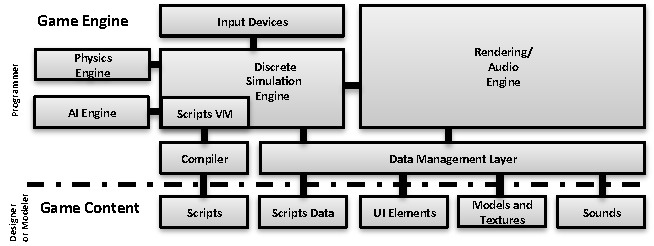
\includegraphics[scale=0.8]{engine_architecture.pdf}
\end{center}
\label{fig:data_driven_games}
\caption{Data-driven engine architecture, from \cite{SGL}}
\end{figure}

Virtual reality browsers face big challenges centered on performance and complexity. Performance is needed because the framerate at which the virtual world is rendered and animated must be high enough to give the user a feeling of smoothness. The scene must be rendered at least at 30 frames per seconds, but higher framerates (e.g. 60 frames per second) are perceived by the user as more pleasant.

Both the visual and logical complexities of a virtual world are very important. Visual richness gives the user the impression of a more realistic and detailed world, with many beautifully rendered objects, while logical complexity permits articulated responses that give the user the feeling of being part of a realistic world with its own set of rules and internal laws.

One of the most important tasks for developers of interactive worlds is to find the right trade-off between these sometimes conflicting requirements. Increasing performance requires a mixture of compromise (reducing the size of the world or ``dumbing down'' its responses) and time-consuming low-level optimization. We believe that automated optimization of interactive applications is a fundamental frontier if we wish to enable developers to build richer worlds without exponentially increasing costs.

Modern 3D browsers and engines are based on a data-driven architecture as shown in Figure \ref{fig:data_driven_games}, taken from \cite{SGL}.

In a data-driven engine the engine contains only general knowledge about virtual worlds, but nothing specific about the peculiar features of a specific virtual world. The specific virtual world will be loaded from the game content in the form of configuration files and scripts. A data-driven engine loads from files two main datasets:

\begin{itemize}
\addtolength{\itemsep}{-0.5\baselineskip}
\item a \textbf{scene}, the set of entities that populate the virtual world
\item \textbf{scripts}, the set of (possibly complex) behaviors that animate the scene entities
\end{itemize}

The scene is composed by a heterogeneous set of entities, each of a different kind. Entities may be virtual characters, trees, 2d or 3d models; entities may also be purely logical and invisible entities such as timers, triggers and proximity sensors.

Scripts give depth to a scene by implementing complex interrelationships between entities. Scripting can be done at three different levels of increasing complexity and expressive power:

\begin{itemize}
\addtolength{\itemsep}{-0.5\baselineskip}
\item \textit{routing} is a simple transmission of values from one entity to another
\item more complex scripts can perform data conversions when moving information between entities
\item even more advanced scripts can create, remove or modify entities of a scene
\end{itemize}

The usual implementation of an engine (see \cite{GAME_OO_HIERARCHY}) features an object-oriented architecture of classes. At the root of this architecture is a class that represents the most generic entity, and from which all other entities are derived. The engine maintains a list of these generic entities, which are all updated and handled through a set of virtual functions. This architecture is a source of often underestimated overhead. Dynamic dispatching is not too costly for a few calls, but when we have many entities, the cost of invoking various virtual functions many times for each frame can become very high. Sometimes the cost of the dynamic dispatching architecture may become higher than the cost of the actual operations being dispatched.

Scripts usually access the scene dynamically. This means that a script must look for the right entities with a mixture of lookups by name and unsafe casts. For example, consider how a Java script may access the \texttt{time} field of a \texttt{myClock} node of type \texttt{timer}:

\begin{lstlisting}
\addtolength{\itemsep}{-0.5\baselineskip}
X3DNode myClock = 
 mainScene.getNamedNode("myClock");
SFTime time = 
  (SFTime) myClock.getField("time");
\end{lstlisting}

This style is unsafe, since \texttt{myClock} may not exist or it may have the wrong type, and it also incurs in significant overhead.

In this paper we will focus exclusively on the X3D language, since it is a recognized standard and it offers a good benchmark to test virtual worlds where we can specify our scene and its various scripts. In the paper we show how we have tackled the problem of increasing performance in X3D browsers while also making scripts safe. We have used a simple compilation technique that removes many unnecessary dynamically dispatched invocations; this technique also allows us to introduce safety for scripts that access the state, so that they do not need to perform unsafe dynamic lookups when searching for specific nodes. To the best of our knowledge, this is the first approach that experiments with compiling X3D scripts and scenes in order to achieve greater performance and safe scripts. None of the previous approaches we are aware of focuses on compilation of X3D as a means to achieve both higher performance (by reducing overhead) and safety (by introducing compile-time checks). Higher performance through compilation includes a long list of research work such as \cite{OPT1,OPT2,OPT3} which has shown that compilation can yield better runtime performance by reducing dynamic overhead and improving other properties of the generated code. Similarly, introducing safety in dynamic languages such as scripting systems has been studied in general in the context of generating typed programs from untyped scripts in \cite{SAFESCRIPTS1}, and the problem of statically typing information which is generally untyped has also been explored in the Haskell community in \cite{SAFESCRIPTS2} among many others.

In Section \ref{sec:solution_workflow} we discuss the general architecture of our system. In Section \ref{sec:compiling_scene} we show how our technique generates the code and the type definitions that represent a scene. In Section \ref{sec:case_study} we show an example of a compiled scene and its routes. In Section \ref{sec:benchmarks} we report some benchmarks that show speed increasing when rendering a sample scene with just nodes and routes by applying our technique. Finally, in Section \ref{sec:compiling_scripts} we discuss how we represent scripts that externally access the scene.




%Problem Statement
\section{Technical challenges in games development}
\label{sec:problem statement}
In this section we introduce the general architecture of a game. We then present an example of common timing and synchronization primitives used in DSL's for games and we show some techniques typically used to implement them. For each technique we list the main drawbacks. Finally we present our solution to the problem of developing a DSL for games.

\subsection{Preliminaries}
A game engine is usually made by several interoperating components. All the components use a shared data structure, called \textit{game state}, for their execution. The two main components of a game are the \textit{logic engine}, which defines how the game state evolves during the game execution, and the \textit{graphics enginge}, which draws the scene by reading the updated game state. These two components are executed in lockstep within a function called \textit{game loop}. The game loop is executed indefinitely, updating the game state by calling the logic engine, and drawing the scene by using the graphics engine. An iteration of the game loop is called \textit{frame}. Usually a game should run between 30 to 60 frames per second. This requires both the graphics engine and the logic engine to be high-performance. In this paper we will only take into account the performance of the logic engine, as scripting drives the logic of the game loop. A schematic representation of this architecture can be seen in Figure \ref{fig:game_loop}.

\begin{figure}
	\centering
	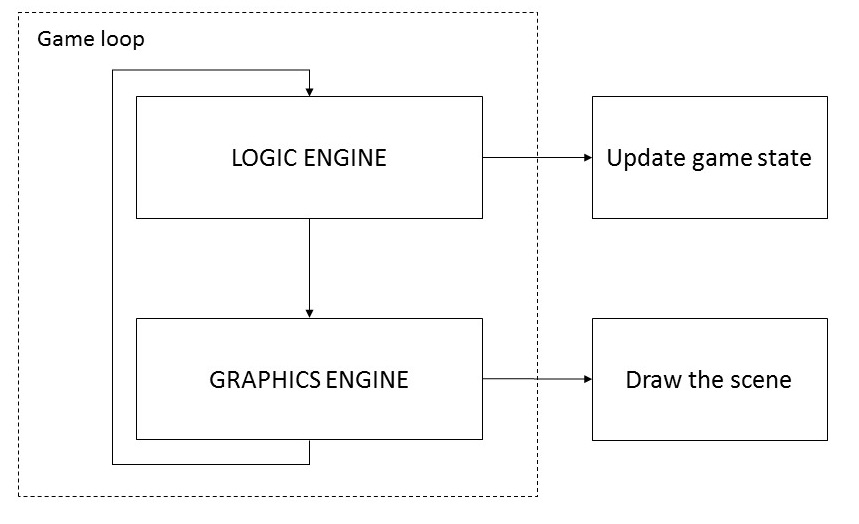
\includegraphics[scale=0.3]{Pictures/game_loop}
	\caption{Game loop}
	\label{fig:game_loop}
\end{figure}

\subsection{A time and synchronization primitive}
\label{subsec:synchronization}
A common requirement in game DSL's is a statement which allows to pause the execution of a function for a specified amount of time or until a condition is met. We will refer to these statements as \texttt{wait} and \texttt{when}. Such a behaviour can be modelled using different techniques:

\begin{itemize}
	\item \textit{Threads} allow to solve such synchronization problems but they are unsuitable for video game development because of memory usage and CPU overhead due to their scheduling.
	\item \textit{Finite State Machines} allow to represent such concurrent behaviours \cite{CASANOVA2_PAPER} by using a \texttt{switch} control structure to an opportune state. For instance in the case of timed wait, the states are \textit{wating} and \texttt{clear} (when the timer has elapsed). This solution is high-performance but the logic of the behaviour is lost inside the \texttt{switch} structure.
	\item \textit{Strategy pattern} allows to represent the instructions of the language has polymorphic data types. Each concurrent structure is implemented by a class which defines the behaviour of the current structure, and the next structure to execute. This solution is not high-performance due to virtuality and the high number of object instantiations.
	\item \textit{Monadic DSL} uses a variation of the state monad. It represents scripts with two states: \textit{Done} and \textit{Next}. The bind operator is used to simulate the code interruption. This approach is simple and elegant but it suffers of the same virtuality problems of the strategy pattern, this time because of the extensive use of lambda expressions.
	\item \textit{Compiled DSL} is the most common solution and allows to represent the concurrency by using concurrent control structures defined in the language. Compiled DSL's grant high-performance and code readability, but they require to implement a compiler or an interpreter for it.
\end{itemize}

In what follows we show a possible implementation of these statements using the presented techniques. We deliberately ignore the thread-based implementation since, as explained above, threads are not suitable for game development.

\paragraph{Monadic DSL:} A possible approach to building an interpreted DSL is using monads in a functional programming language, as done in \cite{CASANOVA1_PAPER}. A script is a function that takes no input parameters and returns the state of the script after the execution of the current statement. The state can be either \textit{Done}, when the script terminates, or \textit{Next} when the script is still running and we need to pass the rest of the script to be evaluated. We present a definition of the monad in the following code snippet in pseudo-ml:

\begin{lstlisting}
type Script<'a> = Unit -> State<'a>
and State<'a> = Done of 'a | Next of Script<'a>
\end{lstlisting}

\noindent
We can define the \texttt{Return} and \texttt{Bind} operators as follow:

\begin{lstlisting}
let return (x : 'a) : Script<'a> =
  fun () -> Done x
  
let (p : Script<'a>) >>= (k : 'a -> Script<'b>) : Script<'b> =
  fun () ->
    match p with
    | Done x -> k x ()
    | Next p' -> Next(p' >>= k)
\end{lstlisting}

\noindent
The \texttt{Return} operator simply returns a script that builds the result of the computation. The \texttt{Bind} operator checks the current state of the script: if the script has terminated then it simply builds the result by executing the last script statement, otherwise it returns the continuation containing the invocation of the \texttt{Bind} on the remaining part of the script. In this framework the \texttt{wait} statement can be implemented as follows (we assume that \texttt{do} is a shortcut for the bind on a function returning \texttt{Script<Unit>}):

\begin{lstlisting}
let yield : Script<Unit> =
  fun () -> Next(fun () -> Done ())

let rec waitRecursion (interval : float32, 
                       startingTime : float32) : Script<Unit> =
  let t = getTime()
  let dt = (t - t0)
  if dt < interval then
    do yield
    do waitRecursion(startingTime)
  else
    return ()
      
let wait (timer : float32) : Script<Unit> =
  let t0 = getTime()
  do waitRecursion(timer, t0)
  
let when (predicate : Unit -> bool) : Script<Unit> =
  if predicate () then return ()
  else
    do yield
    do when predicate
\end{lstlisting}
\noindent
The \texttt{yield} function simply forces the script to stop for one frame. The \texttt{wait} function recursively checks if the timer has elapsed. If this is not the case it skips a frame and then re-evaluates otherwise it returns \texttt{Unit}. \texttt{wait} on a predicate simply skips a frame and keeps re-executing itself until the condition is met.

\paragraph{Strategy pattern} Implementing \texttt{wait} and \texttt{when} with the strategy pattern requires to define an interface which contains the signature for a method to run the script. Usually scripts need to access the time elapsed between the current frame and the previous one and to a reference to the game state data structure for various reasons, which are passed as parameter for this method. The method returns the updated script after the current execution. We present the code for the interface in a pseudo-C\# code:

\begin{lstlisting}
public interface Script
  public Script Run(float dt, GameState state);
\end{lstlisting}

We will then model \texttt{wait} and \texttt{when} with two classes implementing such interface. Each of the script commands contains a reference to the next statement to execute.

\begin{lstlisting}
public class Wait : Statement
  private Statement next;
  private float time;
  
  public Script Run(float dt, GameState state)
    if (time >= 0)
      time -= dt;
      return this;
    else
      return next;

public class When : Statement
  private Func<bool> predicate;
  private Script next;
  
  public Script Run(float dt, GameState state)
    if (predicate())
      return next;
    else
      return this;
\end{lstlisting}

\paragraph{Finite state machines:} In this approach we model \texttt{wait} and \texttt{when} as finite state automata. Both statements require to store the state of the automata. \texttt{wait} requires to store a timer whose value is updated at each frame. \texttt{when} stores a predicate to execute and check at every game logic update. \texttt{wait} has three states: (\textit{i}) timer initialization, (\textit{ii}) check timer and update, and (\textit{iii}) timer elapsed. In the first state we initialize the timer and then update it for the first time. The second state is used to check whether the timer has elapsed. The third state is used to continue with the execution after the time has elapsed.

\begin{lstlisting}
//WAIT
public void Update(float dt, GameState gameState)
  switch(state)
    case -1: 
      this.t = timer;
      state = 0;
      goto case 0;
    case 0:
      this.t = this.t - dt
      if (this.t <= 0)
        state = 1;
        goto case 1:
      else
        return;
    case 1:
    //run the code after wait
\end{lstlisting}

\texttt{when} has two states: (\textit{i}) check predicate, (\textit{ii}) predicate satisfied (go on with the execution). The first state checks if the predicate has been satisfied. If that is the case, we jump to the next state, otherwise we pause the execution and we remain in the same state.

\begin{lstlisting}
//WHEN
public void Update(float dt, GameState gameState)
  switch(state)
    case 0:
      if (predicate())
        state = 1;
        goto case 1:
      else
        return;
    case 1:
    //run the code after when
\end{lstlisting}

\paragraph{Waiting with a hard-coded compiler:} This approach requires to build a compiler by generating the syntax using a standard lexer/parser generator. After that usually it is required to define a set of type rules, and the operational semantics of the language constructs. The type rules and the operational semantics are then implemented in the type checker and the code generator of the compiler.

\subsection{Discussion}
In the previous paragraph we have seen different techniques employed by developers to implement timing and synchronization statements commonly used in video games. We now list the advantages and disadvantages of each solution:

\begin{itemize}
	\item \textit{Monadic DSL:} this solution is elegant but inefficient, because of the extensive use of lambda expressions in monads. Indeed lambdas are usually implemented with virtual method calls. The code to define a monadic DSL is compact.
	\item \textit{Strategy Pattern:} this solution is simple but low-performance because of the virtual method calls the logic update must invoke to run the statements and the high number of object instantiation to generate the script statements (one per statement). Besides the readability of the program for long scripts is lost due to the long chain of object instantiations. A library supporting scripts implemented with the strategy pattern is compact.
	\item \textit{Finite state machines:} this approach is high-performance due to the small overhead of the \texttt{switch} control structure. Unfortunately the logic of the program for very complex scripts with several nested synchronizations is lost inside huge \texttt{switch} structures and the complexity increases drastically with the number of interruptions and synchronizations in the script \cite{AI_GAMES}. Moreover note that for each timer we have to maintain a separate timer, and for any of the two control structures we need to store the state of the automaton. Implementing complex synchronizations require long and complex state machines.
	\item \textit{Hard-coded compiler:} this approach is high-performance, as we could generate the state machines presented above during the code generation step, but building, maintaining, and extending a hard-coded compiler is a hard and time-consuming task. The code length increases with the size of the compiler (in term of modules and code lines) and the language complexity.
\end{itemize}
This situation is summarized in Table \ref{tab:techniques}.

\begin{table}
	\small
	\centering
	\begin{tabular}{|c|c|c|c|}
		\hline
		Technique & Readability & Performance & Code length \\
		\hline
		Monadic DSL & \checkmark & \ding{55} & \checkmark \\
		\hline
		Strategy Pattern & \ding{55} & \ding{55} & \checkmark \\
		\hline
		Finite state machines & \ding{55} & \checkmark & \ding{55} \\
		\hline
		Hard-coded compiler & \checkmark & \checkmark & \ding{55} \\
		\hline
	\end{tabular}
	\caption{Pros and cons of script implementation techniques}
	\label{tab:techniques}
\end{table}

In this work we propose another development approach in building a game DSL by using a metacompiler, a program which takes as input a language definition, a program written in that language, and generates executable code.

\noindent
Given this considerations, we formulate the following problem statement.

\vspace{0.5cm}
\noindent
\textbf{PROBLEM STATEMENT:}
Given the formal definition of a game DSL our goal is to automate, by using a metacompiler, the process of building a compiler for that language in a (\textit{i}) short (code lines), (\textit{ii}) clear (code readability), and (\textit{iii}) efficient (time execution) way, with respect to a hand-made implementation.


%Orch model
%\section{A concurrency model for games}
%\label{sec:orch model}
%In this section we discuss a model for computation which was directly inspired by the ``orchestration model'' \cite{misra2007computation}, and we show how this model simplifies the example above.

\subsection{Our model}
We begin with the observation that components can be treated as independent and concurrent programs.
Our model is tiny since it consists of four operators:  (\texttt{$\rightarrow$}) the bind operator, (\texttt{||}) the parallel operator, (\texttt{$\downarrow$}) the yield operator, and (\texttt{let}) the expression definition operator.

Given two concurrent programs, \texttt{g} and \texttt{f}: \texttt{f$\rightarrow$g} runs \texttt{g} after \texttt{f} has terminated. The expression becomes \texttt{f>g} if we do not want any result of \texttt{f} to enter in the scope of \texttt{g}); \texttt{(f||g)} runs \texttt{f} and \texttt{g} in parallel. \texttt{$\downarrow x$, v} changes the value of v into x (x is a variable defined either as an argument of the current function or a variable defined outside the function itself); \texttt{let} allows the assignment of expressions to labels in the form of \texttt{let name = expr}. The \textit{state} is made up from the definition of all the variables involved in the logic.


\subsection{Re-implementation of the case study}
We now show how our model can express the dynamic of a game by using it to re-write our case study. 
The implementation is divided into three blocks:
\begin{enumerate}
\item \texttt{UPDATE}, implements the logic ;
\item \texttt{DRAW}, draws the entities of the game; 
\item \texttt{GAME}, coordinates the execution of both \texttt{UPDATE} and \texttt{DRAW}.
\end{enumerate}

The new implementation of the game is now given:
In the \texttt{UPDATE} block we define the underlying logic of the game. The key pressure is caught by \texttt{WaitSpacePressed} which waits until the \texttt{space} key is first pressed and then released. The logic of the light switch waits until the space key is pressed, and once this event occurs it turns \texttt{on} the light switch. We turn back to \texttt{off} when we press again the space button. Afterwards, it recurses.
\begin{lstlisting}[caption=LOGIC]
let WaitSpacePressed = 
  wait (Keyboard.Down(Space)) $\rightarrow$
  wait (Keyboard.Up(Space))
let Update sprite_color tick_status = 
  WaitSpacePressed $\rightarrow$
  $\downarrow$ tick_status, Status.Play $\rightarrow$
  $\downarrow$ sprite_color Color.White $\rightarrow$  
  WaitSpacePressed $\rightarrow$
  $\downarrow$ tick_status, Status.Play $\rightarrow$
  $\downarrow$ sprite_color Color.Black $\rightarrow$
  Update sprite_color tick_status
\end{lstlisting}
The \texttt{DRAW} block draws the light switch (which is called \texttt{sprite}) and then recurs.
\begin{lstlisting}[frame=single, caption=DRAW]
let Draw sprite = DrawSprite sprite $\rightarrow$ Draw
\end{lstlisting}
The \texttt{GAME} block loads the light switch sprite (setting its initial color to \texttt{Black}), and runs \texttt{UPDATE} and \texttt{DRAW} in parallel.
\begin{lstlisting}[frame=single, caption=LOOP]]
let sprite = LoadSprite "mySprite.png"
let sound = LoadSoundManager()
let Game = Update(sprite.Color, sound.Status) || 
           Draw(sprite)				
\end{lstlisting}
The spurious constructs used to maintain the state machine are no longer present explicitly, but stored and handled implicitly in the form of \textit{program counters} of the various processes. This is due to the control flow semantics of our model. The resulting program has more in common (from the perspective of readability) with the \textit{definition} of the light switch problem than the program presented in Section 2.


We will now proceed with the definition of the Casanova 2 programming language that is inspired by the concepts of orchestration languages. 

%Casanova 2
\section{Casanova 2}
\label{sec:casanova 2}
Languages, in general, offer more expressive power than engines, because of the possibility to combine and nest the constructs. A language specifically designed and built with game programming in mind can help with common aspects of game development (such as time, concurrency, and state updates) that regular languages do not encompass.
In this regard, we present the language Casanova 2, based on \cite{maggiore2012designing}, which takes its inspiration from the orchestration model of \cite{misra2007computation}. We show how Casanova 2 is designed in particular to express the typical dynamics present in games.

\subsection{The basic idea behind Casanova 2}
An abstraction of a game should be able to represent its main elements, i.e., its state variables and their (discrete and dynamic) interactions.
For this purpose, we built an (intentionally) small programming language of which the main features are \textit{state} and \textit{rules}:
\begin{enumerate}[\itshape(i)]
\item The \textit{state} of a game is represented by a hierarchical type definition. Each node of the hierarchy is called an \textit{entity} (besides the root, which is called \textit{world}). Each entity contains a series of fields that represent primitive types, collections, or even references to other entities. Through access to shared data entities we achieve concurrent coordination.
\item The logic of each entity is defined as a series of implicitly parallel looping code blocks. Each implicit block, called a \textit{rule}, represents a specific dynamic of the entity. A rule represents a dynamic, which can be continuous (simple and effect-free) or discrete (with side-effect, the most important of which is \textit{wait}).
\end{enumerate}
\subsection{Casanova patrol}
We now show how we rewrite the patrol program presented in Section \ref{sec:problem statement} using Casanova 2.
\begin{lstlisting}[caption=Patrol in Casanova 2]
world Patrol = {
   V : Vector2
   P : Vector2
   Checkpoints : [Vector2]

   rule P = P + V * dt

   rule V =
    for checkpoint in Checkpoints do
      yield $\norm{\texttt{checkpoint - P}}$
      wait P = checkpoint
      yield Vector2.Zero
      wait 10<s>
}
\end{lstlisting}

The first three lines within the definition of Patrol describe the game state, containing three variables: the velocity \texttt{V}, the position \texttt{P}, and a checkpoint list \texttt{Checkpoints}. The next line gives the continuous dynamic, namely the rule P which runs once per frame, i.e., at every frame the position \texttt{P} is integrated by the velocity \texttt{V} over \texttt{dt} (a global value supplied by the system that represents the time difference between the current and the previous frame). The remainder of the definition gives the discrete dynamic, namely the rule V, which represents the movement between checkpoints. The checkpoints are traversed in order, and for each selected checkpoint \texttt{checkpoint} we change the value of the velocity in order to move the patrol towards it (\texttt{yield checkpoint - P}). Then, we wait until the patrol reaches the checkpoint (\texttt{wait P = checkpoint}), and once the checkpoint is reached we stop the patrol, by setting its velocity to 0 (\texttt{yield Vector2.Zero}) for 10 seconds (\texttt{wait 10<s>}). At this point the loop continues and a new checkpoint is selected. We reiterate the list again once we have traversed all the checkpoints.

Note that, in general, a game can be considered a series of entities that run in synchronization in order to achieve a specific goal. In Casanova 2 every entity in the state (as well as every rule in an entity) is in essence an \textit{independent} concurrent program \cite{schneider1997concurrent}. Coordination between these programs happens through a shared state.


%Consider the following, based on the Boids algorithm \cite{reynolds1987flocks}, where a group of subordinates are synchronized in order to follow a leader (whose behavior is the same as the patrol presented above).
%\begin{lstlisting} [caption=Boids in Casanova 2]
%entity Subordinate = {
%   Leader   : Patrol
%   Group    : [Subordinate]
%   MaxSpeed : Vector2
%   P : Vector2
%   V : Vector2
%   rule P = P + V * dt
%   rule V =
%    let repulsion =
%       [for p in Group do
%        sumBy Normalize$(\texttt{P} - \texttt{p.P}) * (1 - \sigma(d(\texttt{P}, \texttt{p.P})))$]
%    yield (Normalize$(\texttt{Leader.P} - \texttt{P})$ +
%           Normalize$(\texttt{repulsion})) * \texttt{MaxSpeed}$
%}
%\end{lstlisting}\footnote{$\sigma$ is a sigmoid function, $d$ represents a distance function}

%During execution each subordinate follows the leader, avoiding at the same time collisions with his team-mates.
%This behavior requires synchronization, which is achieved by the rule on the velocity \texttt{V}. We distinguish the leader (\texttt{Leader} of type \texttt{Patrol}) from the group (\texttt{Group} of type \texttt{[Subordinate]}): their behaviors are different, so their rules must be different as well. Given a subordinate, at every iteration we update its position \texttt{P} (by integrating \texttt{P} by \texttt{V} over \texttt{dt}) and its velocity \texttt{V} (computing a repulsion value to try to avoid collisions with other members of the group, and then reducing the gap between the selected subordinate and the leader).

% PS: I do not really understand what this subsubsection is trying to argue. Please make that clear.


\subsection{Syntax}
The syntax of the language (here presented in Backus-Naur form \cite{strings2010backus}) is rather brief. It allows the declaration of entities as simple functional types (records, tuples, lists, or unions). Records may have fields. Rules contain expressions which have the typical shape of functional expressions, augmented with \texttt{wait}, \texttt{yield}, and queries on lists:
\begin{lstlisting}[caption=Casanova 2 syntax]
<Program> ::=
    <moduleStatement> {<openStatement>}
    <worldDecl> {<entityDecl>}

<moduleStatement> ::= module id
<openStatemnt>    ::= open id
<worldDecl>    ::= world id ["("<formals>")"] =
                   <worldOrEntityDecl>
<entityDecl>   ::= entity id ["("<formals>")"] =
                   <worldOrEntityDecl>
<worldOrEntityDecl> ::= "{" <entityBlock> "}"
<entityBlock>  ::= {<fieldDecl>} {<ruleDecl>}
                   <create>
<create> ::= Create "(" {<formals>} ") = <expr>
<formals>   ::= id [":" <type>] {"," <formals>}
<fieldDecl> ::= id [":" <type>]
<ruleDecl>  ::= rule id {"," id} "=" <expr>
<type>      ::= int |boolean  |float |Vector2
                |Vector3 |string |char
                |list "<" <type> ">" |<generic>
                |<type> "[" "]" |id
<generic>     ::= "'" id
<expr> ::= ...(* typical expressions : let, if,
                 for , while , new, etc. *)
           | wait (<arithExpr> | <boolExpr>)
           | yield | <arithExpr> | <boolExpr>
           | <literal> | <queryExpr> | <seq>
<seq>        ::= <expr> <expr>
<arithExpr>  ::= ...//arithmetic expressions
<boolExpr>   ::= ...//boolean expressions
<literal>    ::= ...//strings , numbers
<queryExpr>  ::= ...//query expressions
\end{lstlisting}


\subsection{Semantics}
The semantics of Casanova 2 is \textit{rewrite-based} \cite{klop1990term}, meaning that the current game world is transformed into another one with different values for its fields and different expressions for its rules.
Given a game world $\omega$, the world is structured as a tree of entities. Each entity $E$ has some fields $f_1 \dots f_n$ and some rules $r_1 \dots r_m$.
\begin{lstlisting}[mathescape]
E = { Field$_1$ = f$_1$; $\dots$; Field$_n$ = f$_n$;
      Rule$_1$ = r$_1$; $\dots$; Rule$_m$ = r$_m$ }
\end{lstlisting}
Each rule acts on a subset of the fields of the entity by defining their new value after one (or more) ticks of the simulation. For simplicity, in the following we assume that each rule updates all fields simultaneously.


An entity is updated by evaluating, in order, all the rules for the fields:
\begin{lstlisting}[mathescape]
tick(e:E, dt) =
 { Field$_1$=tick(f$_1^m$, dt); $\dots$; Field$_n$=tick(f$_n^m$, dt);
   Rule$_1$=r$_1'$; $\dots$; Rule$_m$=r$_m'$ }
where
  f$_1^m$, $\dots$, f$_n^m$, r$_m'$ = step(f$_1^{m-1}$, $\dots$, f$_n^{m-1}$, r$_m$)
  .
  .
  f$_1^1$, $\dots$, f$_n^1$, r$_1'$ = step(f$_1$, $\dots$, f$_n$, r$_1$)
\end{lstlisting}
We define the \texttt{step} function as a function that recursively evaluates the body of a rule. The function evaluates expressions in sequential order until it encounters either a \texttt{wait} or a \texttt{yield} statement. It also returns \textit{the remainder of the rule body}, so that the rule will effectively be resumed where it left off at the next evaluation of \texttt{step}:
\begin{lstlisting}[mathescape]
step(f$_1$, $\dots$, f$_n$, {let x = y in r$'$}) =
  step(f$_1$, $\dots$, f$_n$, r$'$[x:=y])

step(f$_1$, $\dots$, f$_n$, {if x then r$'$ else r$''$; r$'''$})
  when (x = true) = step(f$_1$, $\dots$, f$_n$, {r$'$; r$'''$})

step(f$_1$, $\dots$, f$_n$, {if x then r$'$ else r$''$; r$'''$})
  when (x = false) = step(f$_1$, $\dots$, f$_n$, {r$''$; r$'''$})

step(f$_1$, $\dots$, f$_n$, {yield x; r$'$}) = x, r$'$

step(f$_1$, $\dots$, f$_n$, {wait n; r$'$})
  when (n > 0.0) = f$_1$, $\dots$, f$_n$, {wait (n-dt); r$'$}

step(f$_1$, $\dots$, f$_n$, {wait n; r$'$})
  when (n = 0.0) = step(f$_1$, $\dots$, f$_n$, r$'$)

step(f$_1$, $\dots$, f$_n$, {for x in y:ys do r$'$; r$''$})
  step(f$_1$, $\dots$, f$_n$,
       {r$'$[x:=y];
        for x in ys do r$'$; r$''$})

step(f$_1$, $\dots$, f$_n$, {for x in [] do r$'$; r$''$})
  step(f$_1$, $\dots$, f$_n$, r$''$)
\end{lstlisting}

\subsection{Compiler description}
Specific syntax built around the concept of altering the execution flow of a Casanova program allows the Casanova compiler to translate a Casanova program into an equivalent and high performance low-level program with the same semantics. The result is a high performance program made by a single switch structure, without nesting.
A big advantage of this solution is that we may ignore typical software engineering rules, such as readability and code maintainability (as readability and maintainability are only needed for the Casanova specification of the game).

Usually, software engineering implementations are based on a series of nested state machines, but nesting yields a low performance because of the state selection. In contrast, the Casanova compiler produces an inlining of all the nested state machines into a single sound and fast state machine (which code is pretty much unreadable).
% The correct choice of constructs in a Casanova program is fundamental in order to allow the compiler to apply the appropriate transformations. Coding the state machines into Casanova is possible by hand, although difficult as the game increases in terms of dynamics (a series of nested \texttt{if} that mimic the decisions), but no guarantees about correctness and performance can be provided by our tool.





%Evaluation
\section{Evaluation}
\label{sec:evaluation}
GrandeOmega has been tested extensively with students from Hogeschool Rotterdam, a university of applied science in the Netherlands. The classes were divided into two groups: in the first classes were given some programming assignments to be completed in the traditional way (without GrandeOmega), while in the second other classes were asked to solve the assignments both in the traditional way and in GrandeOmega. Table \ref{tab:performance_go} and Figure \ref{fig:bar_chart} contain data relative to the pass rate and average grades of the classes that were asked to used also GrandeOmega, with and without using it. Table \ref{tab:prediction} and Figure \ref{fig:prediction} contain data relative to the accuracy of the prediction on the student success performed by GrandeOmega. The total number of students who participated is 241.

The data shows that the use of GrandeOmega enhanced the pass rate of classes 1B and 1C, but not that of 1F, 1L, and 1A. This means that the students of 1B and 1C failed questions in the traditional way that they were able to solve in GrandeOmega. Nonetheless, we can see that it always enhanced the grades of all the classes by at least 4\%. Moreover, if we compare the average passing grade of these classes with those who never used GrandeOmega, we can see that we reach a difference of even 12\%.

GrandeOmega was revealed to be effective even in predicting the success of students with a total reliability of 77\%, based on the percentage of assignment completed correctly.

\begin{table}[!h]
	\begin{tabular}{|p{0.1\columnwidth}|p{0.1\columnwidth}|p{0.1\columnwidth}|p{0.1\columnwidth}|p{0.1\columnwidth}|p{0.1\columnwidth}|}
		\hline
		\textbf{Class} & Completions & Pass rate & Pass rate G.O. & Average grade & Average grade G.O. \\
		\hline
		INF1B & 71.8 & 3 & 14 & 84.7 & 97.2 \\
		\hline
		INF1F & 56.7 & 6 & 5 & 77.0 & 88.1 \\
		\hline
		INF1L & 48.1 & 2 & 2 & 75 & 83.8 \\
		\hline
		INF1A & 41.7 & 7 & 7 & 82.1 & 86.5 \\
		\hline
		INF1C & 35.6 & 5 & 7 & 82.5 & 93.3 \\
		\hline
	\end{tabular}
	\caption{Student performance before and after GrandeOmega}
	\label{tab:performance_go}
\end{table}

\begin{table}[!h]
	\begin{tabular}{|p{0.2\textwidth}|p{0.2\textwidth}|p{0.2\textwidth}|p{0.2\textwidth}|p{0.2\textwidth}|}
		\hline
		\textbf{Class} & \textbf{Correct prediction} & \textbf{False positive} & \textbf{False negative} & \textbf{Incorrect prediction} \\
		\hline
		INF1B & 16 & 8 & 2 & 10 \\
		\hline
		INF1F & 11 & 2 & 4 & 6 \\
		\hline
		INF1L & 18 & 3 & 1 & 4 \\
		\hline
		INF1A & 13 & 0 & 2 & 2 \\
		\hline
		INF1C & 15 & 1 & 1 & 2 \\
		\hline
	\end{tabular}
	\caption{Prediction of student performance}
	\label{tab:prediction}
\end{table}

\begin{table}[!h]
	\begin{tabular}{|p{0.25\textwidth}|p{0.25\textwidth}|p{0.25\textwidth}|p{0.25\textwidth}|}
		\hline
		\textbf{Class} & \textbf{Average grade} & \textbf{Passed students} & \textbf{Avarage passing grade} \\
		\hline
		INF1H & 41.4 & 3 & 83.3 \\
		\hline
		INF1E & 30.6 & 1 & 75 \\
		\hline
		INF1J & 23.3 & 0 & N.A. \\
		\hline
		INF1G & 41.4 & 7 & 80.3 \\
		\hline
	\end{tabular}
	\caption{Results of classes without GrandeOmega}
	\label{tab:performance_no_go}
\end{table}

\begin{figure}[!h]
	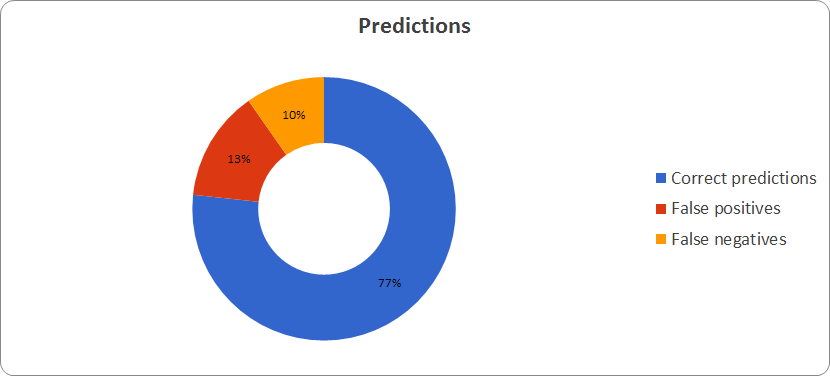
\includegraphics[width = \columnwidth]{Figures/prediction}
	\caption{Predition accuracy of GrandeOmega}
	\label{fig:prediction}
\end{figure}

\begin{figure}[!h]
	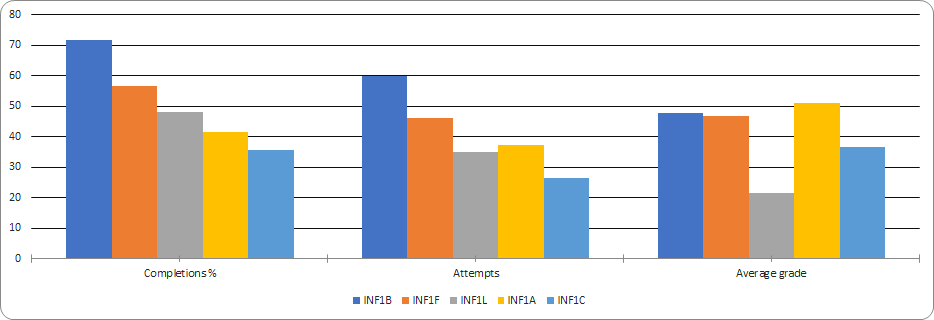
\includegraphics[width = \columnwidth]{Figures/bar_chart}
	\caption{Student performance with and without G.O.}
	\label{fig:bar_chart}
\end{figure}


%conclusions
%%%%%%%%%%%%%%%%%%%%%%%%%%%%%%%%%%%%%%%%%%%%%%%%%%%%%%%%%%
% conclusions.tex
%%%%%%%%%%%%%%%%%%%%%%%%%%%%%%%%%%%%%%%%%%%%%%%%%%%%%%%%%%

Scripts are an important and pervasive aspect of computer games. Scripts simplify the interaction with computer game engines to the point that a designer or an end-user can easily customize gameplay. Scripting languages must support coroutines because these are a very recurring pattern when creating gameplay modules. Scripts should be fast at runtime because games need to run at interactive framerates. Finally, the scripting runtime should be as modular and as programmable as possible to facilitate its integration in an existing game engine.

In this paper we have shown how to use meta-programming facilities (in particular monads) in the functional language F\# to enhance the existing scripting systems which are based on Lua, the current state of the art, in terms of speed, safety and extensibility. We have also shown how having a typed representation of coroutines promotes building powerful libraries of combinators that abstract many common patterns found in scripts. As evidence of the capabilities of our proposed system we have outlined a series of applications of our scripts into an actual game that is under development.


\bibliographystyle{abbrv}
\bibliography{Sections/References}
\end{document}
